\begin{frame}[fragile]
  \frametitle{遇到的问题}
  \framesubtitle{背景介绍}

  在“用户画像”数据的读取中,使用了一个由同事开发的工具,通过接口来读取由由定位团队挖掘出来的用户 “家和公司” 的位置。 
  \vspace{\baselineskip}

  由于接口使用了  pbrpc 协议,所以无法通过简单地方式访问,所以我们使用了导航团队同事开发的一个工具(bin,无源码)来读取数据,然后通过脚本去处理该工具输出的方式来协作。 
  \vspace{\baselineskip}

  \pause
  在脚本运行之后,我们拿到了这样一些结果

\end{frame}

\begin{frame}[fragile]
  \frametitle{日志格式}
  \framesubtitle{背景介绍}
  \begin{verbatim}
    cuid:("武汉市","厦门市","重庆市","上海市","广州市","深圳市","成都市","杭州市")
    cuid:00000000000000000000000000000000
    1 10000000.000000 3000000.000000
    0 10000000.000000 3000000.000000
    cuid:00000000000000000000000000000001
    cuid:00000000000000000000000000000002
    cuid:00000000000000000000000000000003
    1 10000000.000000 3000000.000000
  \end{verbatim}
\end{frame}

\begin{frame}[fragile]
  \frametitle{日志格式}
  \framesubtitle{背景介绍}
  由于对应的工具,并没有详细的文档介绍,我们只能通过同事介绍,这份日志的格式做如下描述:

  
  \begin{itemize}
  \item 日志的第一行,是一些 debug 信息
  \item 日志第二行开始,是一系列的 cuid 的查询结果
  \item[-] 以 cuid 开始的行,表示一个结果的开始
  \item[-] 以``1'' 开始的行,表示用户``家'' 的查询结果
  \item[-] 以``0'' 开始的行,表示用户``公司'' 的查询结果
  \item[-] 未附有查询结果的 cuid, 表示未找到对应的值
  \end{itemize}
\end{frame}

\begin{frame}[fragile]
  \frametitle{状态机}
  \framesubtitle{背景介绍}
  对于这样一份看起来很规则很简洁的日志,我们看看它的状态机是什么样的: \pause
  \begin{figure}[htbp]
    \centering
    \includegraphics[scale=.4]{imgs/log_state_trans.png}
    \caption{日志状态机}
    \label{fig:loc-trans}
  \end{figure}
\end{frame}

\begin{frame}[fragile]
  \frametitle{日志处理}
  \framesubtitle{背景介绍}
  可以看出,即使是很简单的日志文件,它的状态机画出来,也会有很多的边界 case 需要关注。
  \begin{figure}[htbp]
    \centering
    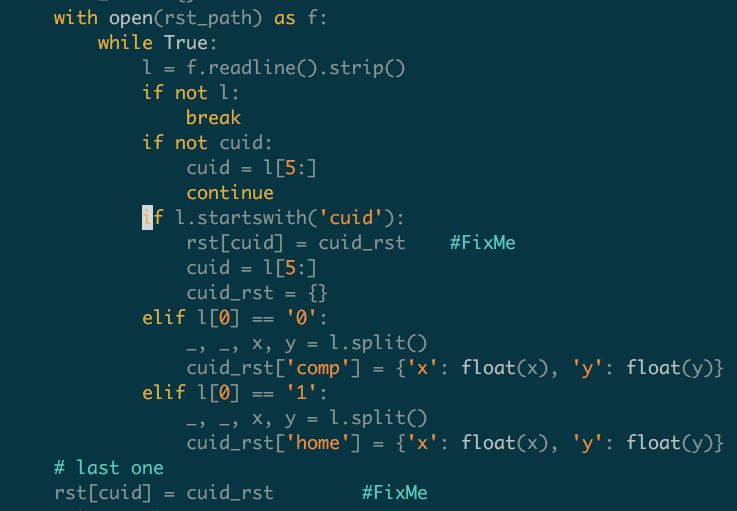
\includegraphics[scale=.3]{imgs/py-regular.png}
  \end{figure}
\end{frame}

\begin{frame}[fragile]
  \frametitle{Cons}
  \framesubtitle{背景介绍}
  根据状态机直接编写处理程序,会遇到以下问题:
  
  \begin{itemize}
  \item 在规则比较复杂的时候,对应的程序有太多分支要处理
  \item 规则很小的变化,可能导致程序变动很大
  \item 很多“可选项”(比如用户家和公司的地址可能不存在)会让程序变得很长
  \item 混合了文本处理与“规则”本身的处理,没有响应介绍不太容易维护
  \end{itemize}
\end{frame}

\begin{frame}[fragile]
  \frametitle{一个 parser 介绍}
  \framesubtitle{Parser}
  下面是另一种“文本”的处理方式: mysql 描述 ``alter database'' 的方式:
  
  \begin{verbatim}
    ALTER {DATABASE | SCHEMA} [db_name]
    alter_specification ...
    ALTER {DATABASE | SCHEMA} db_name
    UPGRADE DATA DIRECTORY NAME

    alter_specification:
    [DEFAULT] CHARACTER SET [=] charset_name
      | [DEFAULT] COLLATE [=] collation_name
  \end{verbatim}
\end{frame}

\begin{frame}[fragile]
  \frametitle{BNF}
  \framesubtitle{Parser}

  Mysql 的文档中,使用了 “BNF” 来描述 sql 的语法,可以把很复杂的、难以表述清楚的规则,完整、清晰的描述,同时保持了简洁。

  \vspace{\baselineskip}

  下面我们尝试使用同样的方式来描述一下前面我们处理的日志
  
\end{frame}

\begin{frame}[fragile]
  \frametitle{BNF}
  \framesubtitle{Parser}
  \begin{verbatim}
    debug_info cuid_rsts

    debug_info:
    cuid:rest_of_line

    cuids_rsts:
    cuid_rst | cuid_rst cuid_rsts
    
    cuid_rst:
    cuid: cuid_value [home_rst [company_rst]]
    
    home_rst:
    1 x_value y_value
    company_rst
    0 x_value y_value
  \end{verbatim}
\end{frame}

\begin{frame}[fragile]
  \frametitle{SSH 简介}
  \framesubtitle{基础应用}
  shell? \pause

  与 Core 相对应,提供用户使用界面 \\ \pause
  \vspace{\baselineskip}
  SSH
  \begin{itemize}
  \item 全称是\textbf{Secure Shell}(VS. Telnet)
  \item 为远程登录会话和其他网络服务提供安全性的协议
  \item 对所有传输的数据进行加密
  \item 创建在应用层和传输层基础上的安全协议(git, scp, rsync, sftp)
  \item 为计算机上的Shell提供安全的传输和使用环境
  \end{itemize}
\end{frame}

\begin{frame}[fragile]
  \frametitle{使用与配置}
  \framesubtitle{基础应用}
  需要在 Server 端运行 \textbf{sshd}
  \begin{itemize}
  \item \verb|openssh-server|
  \item 默认运行在端口 22
  \item 可能使用跳板机
  \item 可能禁止密码登录
  \item 可能禁止 \textsf{root} 登录
  \item 有定制化的登录提示
  \end{itemize}
\end{frame}


\begin{frame}[fragile]
  \frametitle{使用与配置}
  \framesubtitle{基础应用}
  \begin{figure}[htbp]
    \centering
    \includegraphics[scale=.4]{imgs/ssh-splash.png}
    \caption{SSH welcome message}
    \label{fig:ssh-splash}
  \end{figure}
\end{frame}


\begin{frame}[fragile]
  \frametitle{使用与配置}
  \framesubtitle{基础应用}

  \textbf{ssh user@host}

\end{frame}

\begin{frame}[fragile]
  \frametitle{进阶配置}
  \framesubtitle{基础应用}
  使用 ``ssh user@host'' 会遇到诸多不便,例如:
  \begin{itemize}
  \item 不想每次输入密码
  \item 服务器太多,记不住 IP、域名
  \item 由于服务器配置不同,导致用户名、端口不一致
  \item GUI 界面不能使用
  \end{itemize}
\end{frame}

\begin{frame}[fragile]
  \frametitle{密钥登录}
  \framesubtitle{基础应用}
  使用密钥登录的方式,可以避开每次输入密码的烦恼,也更加安全
  \begin{itemize}
  \item 使用``ssh-keygen -t rsa''生成一对密钥
  \item 将公钥``id\_rsa.pub''写入Server 端``\~/.ssh/authorized\_keys''
  \item 修改私钥``id\_rsa'' 的权限
  \item ``ssh user@host''
  \end{itemize}
\end{frame}

\begin{frame}[fragile]
  \frametitle{\~/.ssh/config}
  \framesubtitle{基础应用}
  使用密钥登录之后,只是(可能)免去了输入密码的烦恼 \\
  其他问题怎么解决呢? \\
  \vspace{\baselineskip}
  \pause
  答案在``\~/.ssh/config''中
  \begin{lstlisting}[language=bash]
    Host vm
        HostName 127.0.0.1
        Port 28022
    Host kaikai
        HostName 106.185.43.198
        User lichao
    Host *
        ControlMaster auto
        ControlPath ~/.ssh/%h-%p-%r
        ControlPersist yes
  \end{lstlisting}
\end{frame}

\begin{frame}[fragile]
  \frametitle{X11}
  \framesubtitle{基础应用}

  可以使用 X11 Forwarding 来使用服务器上 GUI 程序
  \begin{itemize}
  \item 服务端开启``X11Forwarding''
  \item 登录用户在使用X11(设置``DISPLAY''环境变量)
  \item ssh -X
  \item 网络足够快
  \end{itemize}
\end{frame}


\begin{frame}[fragile]
  \frametitle{Remote Command}
  \framesubtitle{基础应用}

  有时候我们需要在远程机器上执行一个指令后退出(并且希望执行的结果输出到本地终端上), 可以这样使用 SSH:

  \vspace{\baselineskip}
  ssh user@host ``command''
  \vspace{\baselineskip}

  \pause
  比如去服务器上查找某一个特定的 logid, 可以在多台机器上执行:
  \vspace{\baselineskip}
  ssh lichao06@tc-map-mobile00.tc ``cat log \textbar{} grep \$logid''

\end{frame}

\begin{frame}[fragile]
  \frametitle{Force Remote Command}
  \framesubtitle{基础应用}

  \textbf{同样可以为每个用户单独指定一个成功登录时的指令} \pause

  在``\~/.ssh/authorized\_keys''的公钥前,可以为用户增加不同的设置 \pause \\
  command=``show me the money'' 可以指定用户登录时执行的命令 \pause 
  \vspace{\baselineskip}

  例如:
  \begin{figure}[htbp]
    \centering
    \includegraphics[scale=.4]{imgs/remote-cmd.png}
    \label{fig:ssh-remote-cmd}
  \end{figure}
\end{frame}


\begin{frame}[fragile]
  \frametitle{Force Remote Command}
  \framesubtitle{基础应用}

  作用是? \\
  \vspace{\baselineskip}
  \pause

  e.g.

  当你执行: \\
  \vspace{\baselineskip}
  \verb|git clone git@github.com:lisztli/homework.git|  \\
  \vspace{\baselineskip}
  的时候,其实是执行了: \\

  \vspace{\baselineskip}
  \verb|# ssh git@github.com -- git-receive-pack lisztli/homework.git|\\
  \pause

  \vspace{\baselineskip}
  GitHub 为每个用户的公钥增加了一个``command=xxx'',确保用户可以执行的指令限制在一个白名单之内
\end{frame}



